%%%%%%%%%%%%%%%%%%%%%%%%%%%%%%%%%%%%%%%%%%%%%%%%%%%%%%%%%%%%%%%%%%%%%%%%%%%
%% Trim Size: 9.75in x 6.5in
%% Text Area: 8in (include Runningheads) x 5in
%% ws-m3as.tex   :   28-9-2018
%% Tex file to use with ws-m3as.cls written in Latex2E.
%% The content, structure, format and layout of this style file is the
%% property of World Scientific Publishing Co. Pte. Ltd.
%% Copyright 2018 by World Scientific Publishing Co.
%% All rights are reserved.
%%%%%%%%%%%%%%%%%%%%%%%%%%%%%%%%%%%%%%%%%%%%%%%%%%%%%%%%%%%%%%%%%%%%%%%%%%%%
%

\documentclass{ws-m3as}

\usepackage{times}

\usepackage{indentfirst}

\usepackage{setspace}

\usepackage{float}

\usepackage{amsmath}

\usepackage{multirow}

\begin{document}
	
\markboth{Borges, Diogo S.; 
	Costa-Félix, R.P.B. and Lava, Deise D.}{A Methodology Proposal for Aging Analysis in Systems Based on Uncertainty Propagation and Principal Component Analysis}

%%%%%%%%%%%%%%%%%%% Publisher's Area please ignore %%%%%%%%%%%%%%%%%%%%%%%
%
\catchline{}{}{}{}{}
%
%%%%%%%%%%%%%%%%%%%%%%%%%%%%%%%%%%%%%%%%%%%%%%%%%%%%%%%%%%%%%%%%%%%%%%%%%%

\title{\textbf{A Methodology Proposal for Aging Analysis in Systems Based on Uncertainty Propagation and Principal Component Analysis}}

\author{Diogo da Silva Borges\footnote{Instituto Nacional de Metrologia, Qualidade e Tecnologia (INMETRO) - Av. Nossa Sra. das Graças, 50 - Xerém, Duque de Caxias - RJ, 25250-020, Brazil}}

\address{\textit{LABUS, INMETRO, Av. Nossa Sra. das Graças 50 - Xerém\\ 
Rio de Janeiro, Duque de Caxias 25250-020, Brazil \footnote{Laboratório de Ultrassom, Instituto Nacional de Metrologia, Qualidade e Tecnologia, Avenida Nossa Senhora das Graças 50 - Xerém, Duque de Caxias, Rio de Janeiro, Brasil, diogosb@outlook.com}}\\ diogosb@outlook.com}

\author{Rodrigo Pereira Barretto da Costa Félix}

\address{LABUS, INMETRO, Av. Nossa Sra. das Graças 50 - Xerém\\
Rio de Janeiro, Duque de Caxias 25250-020, Brazil\\
rpfelix@inmetro.gov.br}

\author{Maria de Lourdes Moreira}

\address{SETER, IEN, Rua Hélio de Almeida 75, Cidade Universitária - Ilha do Fundão\\
	Rio de Janeiro, Rio de Janeiro 21941-972, Brazil\\
	malu@ien.gov.br}

\author{Deise Diana Lava}

\address{INMETRO, Av. Nossa Sra. das Graças 50 - Xerém\\
Rio de Janeiro, Duque de Caxias 25250-020, Brazil\\
deise\_dy@hotmail.com}

\maketitle

\begin{history}
\received{(Day Month Year)}
\revised{(Day Month Year)}
%\accepted{(Day Month Year)}
\comby{(xxxxxxxxxx)}
\end{history}

\begin{abstract}
The analysis of systems aging has a fundamental role in quality assurance and the reliability of processes and operations. Thus, the adoption of methodologies capable of predicting the availability of systems susceptible to aging is essential. The present paper aims to present a method capable of predicting a system's behavior based on its degradation caused by aging. For this, predictive and statistical analysis techniques should be used, such as Faul Tree and Fussel Vesely Techniques, Principal Component Analysis and the Monte Carlo Method. As a result of the proposal, the paper presents results capable of detailing the behavior of a system, adopted as an example application case, as well as the contribution of its components to its unavailability, according to Weibull's Probability Density Function. The proposed methodology and the analysis consider the uncertainties associated with the variables of interest, which is a determining factor in quantifying the probability of systems failure. Its relevance is directed towards aging studies, disclosing a straightforward way for research and applications in installations that require high reliability of equipment and systems.	
	
\end{abstract}

\keywords{Faul Tree; PCA; Monte Carlo; Aging.}

\ccode{AMS Subject Classification: 62H22, 62L10, 62P30}

\section{Introduction}	

The need to assess the reliability of systems over time of operation is intrinsic to quality assurance and control. The concern in determining the characteristics of a system susceptible to aging demonstrates aspects inherent to the safety of its operation and maintenance concerning its precision and trueness. Besides, efficient management of aging allows the determination of maintenance routines virtually, directly impacting costs, reliability and availability.  Based on this, it is essential to point out that aging is an agent capable of degrading a system's components. It can cause deterioration in component insulation, damage by fatigue in mechanical parts and erosion in metal structures \cite{WenyuanLi2006}. 

The qualitative and quantitative aspects of the stages that make up the life cycle of systems and components are described employing a hazard function, whose outcome is consolidated in a distribution pattern known in the literature as the bathtub model \cite{Klutke2003} (Fig.\ref{fig:1}).
\begin{figure} [H]
	\centering
	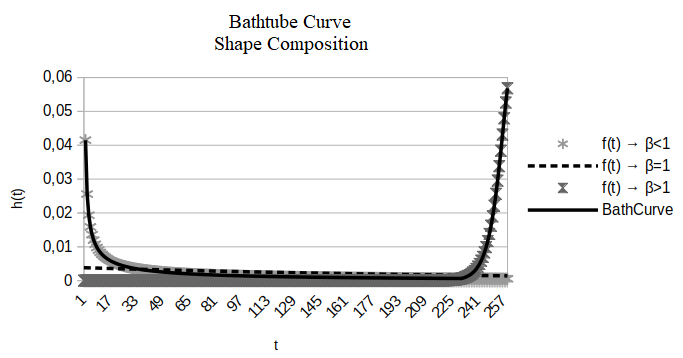
\includegraphics[width=0.7\linewidth]{Figures/BathCurve2}
	\caption{Bathtub Based $\beta$ (Elaborated by the author)}
	\label{fig:1}
\end{figure}

The region of most significant impact for a system concerning the risk of unavailability or loss of function originates when its components' failure rates are in the part of exponential increase (see Fig.\ref{fig:1}). 

Issues related to the analysis of system failures refer to the concern with what is defined as a risk. ``Risk is usually defined as the combination of the probability of occurrence of harm and the severity of that harm" \cite{Matsuoka2012}.

The failures associated with the effects of aging point to dangers arising from the use of systems over time, which have a close relationship with potential damage.  In this sense, the threat is a potential source of unwanted consequences, such as loss of accuracy (e.g., loss of precision and trueness \cite {VIM2012}), unexpected operational deviations and loss of function, for example.

Based on what has been exposed, the present paper aims to carry out a methodological approach capable of being used in the failure analysis of systems. To this, it is proposed to use known techniques for failure analysis and the development of predictive models. In order to fulfill this objective, a methodological approach shall be carried out considering the use of the Fault Tree (FT) technique, pre-processing, Principal Component Analysis (PCA), use of statistical indicators and considerations related to the uncertainties arising from the determination of the failure rate, which shall be processed using the Monte Carlo method (MC). As an application example, an electronic circuit developed for amplifying low voltage signals will be considered.


\section{Theoretical Background}

The methodology for the analysis of aging is formulated based on methods, concepts and techniques known for assessing uncertainty and failures, such as Weibull distribution, FT technique, PCA, MC method and propagating uncertainty techniques. Thus, the realization of a theoretical approach is essential for understanding and using these devices in the composition of aging methodology, presented in the following subsections.


\subsection{Considerations for Using the Fault Tree Technique}

The FT technique makes it possible to characterize the failure probability of a system or equipment by considering the probabilistic analysis of the individual components present (events) associated with independent failures. The technique's working mechanisms consist of propagating probabilities through mathematical relationships between components (gates) \cite{Borges2015}.

The mathematical modeling of the failure of a system, using the FT technique, is done through Boolean logic. Additionally, there is a need for in-depth and detailed knowledge of the object of study. In this way, an FT carries an intrinsic knowledge of the functioning of a system  considered in failure analysis.

The propagation of faults in an FT is carried out mathematically through the relationship between the events, conveniently treated employing literal modeling. This approach makes it possible to use essential simplifications for the model's processing, mainly by considering the concept of minimal cutsets.

The fault tree processing must rely on the concept of minimal cutsets, which represents the maximum simplification that can be performed in the FT methodology. Such simplification can be achieved through simplifications used in Boolean Algebra.

\subsection{Weibull Distribution}

The Weibull distribution has excellent applicability in relation to the study of component life \cite{Lai2006}. The distribution can describe failures in three periods of importance: Infant Mortality, Random Failures and Wear Failures. These regions are characterized by periods of exponential decrease in failure rates, constant failure rates and exponential increase in failure rates, respectively.

The Probability Density Function (PDF) for Weibull Distribution can be used to determine the probability of failure of each component of a system for the three periods described above. It is worth mentioning that this parameter should be input to the methodology of analysis of systems aging. Eq.\ref{eq:3.5} gives Weibull's PDF \cite{Rinne2008}.

\begin{equation}\label{eq:3.5}
f(t)=\frac{\beta}{\eta}\left(\frac{t-\gamma}{\eta}\right)^{\beta-1}\exp-\left(\frac{t-\gamma}{\eta}\right)^{\beta}; \hspace{2pt} for \hspace{2pt} \beta > 0\hspace{2pt},\hspace{2pt} \eta > 0 \hspace{2pt} and \hspace{2pt} t \geq \gamma.
\end{equation}
Where:
\begin{itemlist}
\item $\beta$ is the shape parameter (or slope);
\item $\eta$ is the scale parameter, or characteristic life;
\item $\gamma$ is the location parameter (or failure free life); and
\item $t$ is the analysis time.
\end{itemlist}	

There is the possibility to analyze the failure of a system for a given period of interest, which is identified by varying the parameter $\beta$. The Infantile Mortality  region is provided by $\beta<1$, Random Failures by $\beta=1$ and the Wearout Failures region by $\beta>1$. 

\subsection{Monte Carlo Method and Uncertainty Propagation}

MC method presents itself as a mathematical-statistical tool commonly used in the exact sciences to perform simulations \cite{Yoriyaz2009} with a more exciting bias for highly complex approaches.

The propagation of uncertainties must be made by considering the deviations from the failure rates of each component. Such considerations should be made for all sources of uncertainty associated with determining an exact failure rate value \cite{VIM2012}. Thus, the following steps must be followed for the correct realization of propagation of uncertainties:

\begin{romanlist}[(ii)]
	
\item \textbf{Determination of uncertainty sources:} The sources of uncertainty are characterized as mechanisms responsible for the variation in the realization  of a measurand. Thus, numerous factors can be responsible for these changes, such as environmental conditions, calibration resolution of equipment, systematic error and adjustments, for example.

\item \textbf{Determination of the uncertainty types:} The associated uncertainties can come from two characteristic sources of determining uncertainties \cite{VIM2012}: 

\begin{itemlist}
	
\item \textbf{Type A uncertainty:} All uncertainties that can be obtained through statistical analysis; and 
\item \textbf{Type B uncertainly:} All uncertainties that are characterized by any method other than statistical analysis. 
\end{itemlist}

\item \textbf{Calculation of standard uncertainty:} For an input quantity $X_{i}$  determined by $n$ repeated and independent observations $X_{i}$, $k$, the standard uncertainty $u(x_{i})$ of its estimate $x_{i}=\overline{X}_{i}$ is $u(x_{i})=S(\overline{X}_{i})$, with $S^{2}(\overline{X}_{i})$ is calculated according to \cite{GUN2008}:

\begin{equation}
S^{2}(\overline{q})=\frac{1}{n^{2}-n}\sum_{j=1}^{n} (q_{j}-\frac{1}{n}\sum\limits_{k=1}^{n}q_{k})^{2}
\end{equation}

Where:

\begin{itemlist}
	\item $S^{2}(\overline{q})$ is the experimental variance of the mean; 
	\item $n$ indicates the number of observations; and
	\item $q$ represents the random variable (definition of a random variable in \cite{GUN2008}).\\
\end{itemlist}

Regarding Type B uncertainties, quantification is obtained through from \cite{GUN2008}: Data previous measurements, experience with or general knowledge of the behavior and properties of relevant materials and instruments, manufacturer specifications, data provided in calibration certificates and manuals. Thus, the determination of the standard uncertainty associated with Type B must take into account the type of distribution related to determining deviations in values, such that:

\begin{equation} \label{eq:4.3}
u(x_{i})= \frac{u_ i \left(amostral \right)} {S_i \left( theory \right)}
\end{equation}

Where:

\begin{itemlist}
\item $u_ i\left(amostral\right)$ represents Type B uncertainty; and 
\item $S_i \left( theory\right)$ is the standard deviation of the distribution. In a practical way, $S_i \left( theory\right)$ can be obtained by considering Tab.\ref{table:1}.

\begin{table}[H] 
	\caption{Type B Standard-Uncertainty$^{a}$}
	\label{table:1}
	\begin{center}
		\resizebox{125mm}{!}{
			{\begin{tabular}{@{}ccp{8cm}@{}}\toprule\\
					Distribution & $S_i \left( theory \right)$ & Uncertainly Description \\\\
					\colrule\\
					Rectangular\hphantom{0} &\hphantom{0}$S_i=\frac{b-a}{\sqrt{3}}$ &\hphantom{}Only the maximum and minimum variation values are known (e.g., $a$ and $b$).\\\\
					Triangular \hphantom{0} & \hphantom{0}$S_i=\sqrt{6}$ &\hphantom{}Maximun and minimun values are know (e.g.,$\pm a$) and the most likely value.\\\\
					Normal or t-student$^{b}$ \hphantom{0} &\hphantom{0}$S_i=\delta^{c}$ & \hphantom{}Uncertainty from calibrations and standards.\\\\
					\botrule
		\end{tabular}}}
	\end{center}
	\footnotesize{$^{a}$ Table based in \protect\cite{GUN2008}.}\\
	\footnotesize{$^{b}$ According to the calibration certificate.}\\
	\footnotesize{$^{c}$ Obtained through the inverse two-tailed t-student function considering a level of coverage and the degree of freedom involved.}
\end{table}
\end{itemlist}

\item \textbf{Calculation of expanded uncertainty:} The expanded uncertainty calculation should be performed using the MC method in line with the proposed system aging analysis.

\end{romanlist}

\subsection{Interpretation and Data Visualization Techniques}
Techniques for analyzing and interpreting the data can be used for aging analysis. Through them. it becomes possible to identify the behavior of the system and its components considering aging. PCA and Fussel-Vesely techniques can be used for this purpose. 

The integration between the techniques allows the creation of an "additive model", which can be used to build the predictive model. A large number of data may be necessary to determine a more accurate model. However, it is more practical than performing calculations associated with component failures through the MC method.

\subsection{Fussel-Vesely Technique} 

The FV technique allows identifying the contribution of each component to the unavailability of a system. The technique is related to the direct effect of component failures for the unavailability of a system. In this sense, each component's participation is determined through the proportion of its failure probabilities to the system, that is, its components \cite{Shadiah2019}. Given this, the participation of each component can be quantified through the Eq.\ref{eq:5.1}.

\begin{equation} \label{eq:5.1}
FV=\frac{P(base)-P(x_{i}=0)}{P(base)}
\end{equation}

Where:

\begin{itemlist}
	\item $P(base)$ refers to the probability of the top event (system unavailability) for the base case, which is computed using the actual failure probabilities of all components in the system. The variable in question refers to the calculation of the FT without any change being made to the values of probabilities of failure and associated uncertaintie; and
	\item $P(x_{i}=0)$ is the probability when component is assumed to work without fail. In this case, the probability of failure and associated uncertainty of the component is assumed to be zero, e.g., $P(x_{i}=0)=0$ and $U=0$.
\end{itemlist}

The FV technique generates a parameter of relevance to the aging methodology, which is essential in the participation of Probabilistic Failure Analyzes (PSA). Through the defense-in-depth requirement, the study of failures relates to traceability with system components' behavior \cite{vanderBorst2001}, which makes the FV technique an essential participation tool in your analysis.

\subsection{Principal component analysis}

PCA presents itself as a tool for analyzing multivariate statistical data. It is possible to analyze a set of data using new orthogonal variables called main components and show patterns of similarity in point maps \cite{Mishra2017}. An example of reduction is shown in Fig.\ref{fig:5}.

\begin{figure}[H]
	\centering 
	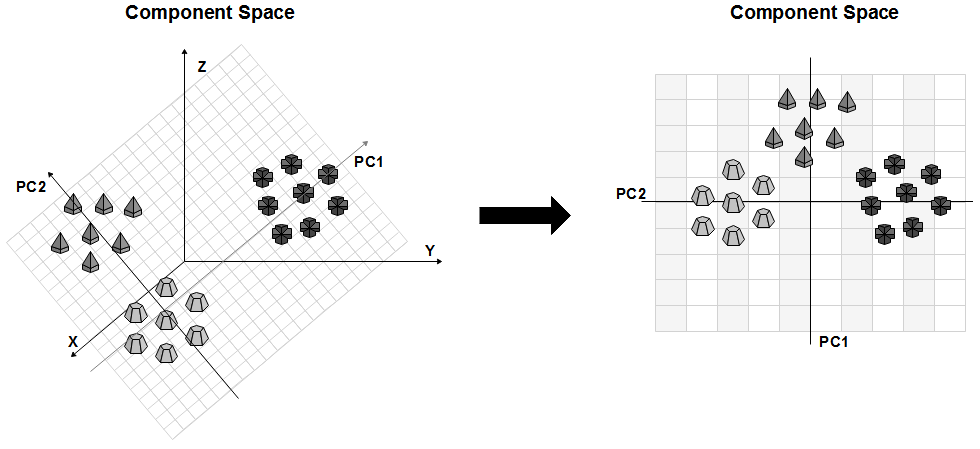
\includegraphics[width=0.9\linewidth]{Figures/PCAExample2}
	\caption{PCA Dimension Reduction Example (Based on \protect\cite{Adcock2015}).}
	\label{fig:5}
\end{figure}

The objective of the technique is to determine a dimensional space ($\Theta$) that can be used to transform data $x={x_{1},x_{2},...,x_{n}}$ of a large dimensional space $R^{M}$ for a smaller dimensional space $R^{k}$, where $n$ represents the total number of samples or observations and $x_{i}$ represents $i^{th}$ sample, pattern, or observation. All samples have the same dimension $x_{i} \in R^{M}$ \cite{Tharwat2016}. Consequently, PCA makes it possible to reduce the size of a data set while retaining as much of the present variation as possible.

\section{Materials and Methods}

The techniques presented throughout this paper should be combined to result in the desired aging methodology. Therefore, it should be used as follows:

\begin{romanlist}[(ii)]
	\item \textbf{Fault Tree Construction:}
	The system should be modeled utilizing intrinsic and in-depth knowledge about its functioning. The development of the FT requires knowledge about the system behavior for each failure mode considered. The failure modeling result depicts the system's behavior for each predicted anomaly. For more complex systems, it may be necessary to form an integration group to determine the real action between the components for a given task. 
	\item \textbf{Mathematical Processing:} The MC method shall be used to analyze system unavailability over time. The technique allows calculations of the probability of failure of the component based on the propagation of uncertainties. In this way, it becomes possible to consider the uncertainties in all the calculation phases.
	\item \textbf{Components study:} The analysis of the components concerning aging is done using the FV technique. Also, the PCA should be used to perform a more perceptual analysis regarding the system's behavior about its components and aging.
\end{romanlist}
 
To create a strategy for applying the aging analysis methodology, Fig.\ref{fig:6} presents a flow chart of the methodology's application. The flowchart contains the sequential steps required to perform an aging analysis from the proposed methodology's perspective.

\begin{figure} [H] 
	\centering 
	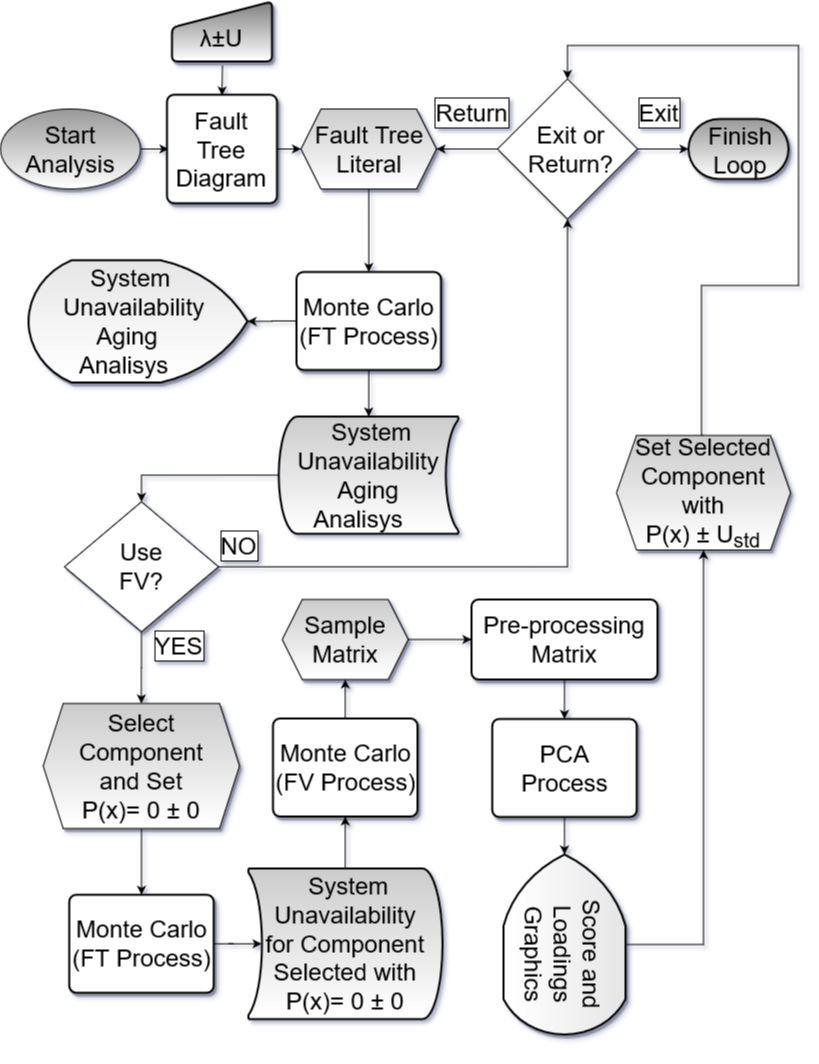
\includegraphics[width=0.8\linewidth]{Figures/Fluxograma}
	\caption{Aging Analysis Methodology Flow Chart (Elaborated by the author)}
	\label{fig:6}
\end{figure}

It is worthwhile mentioning that in Fig.\ref{fig:6}, $\lambda$ represents the probability of component failure; $U_{std}$, the standardized uncertainty and $P(x)$ the failure probability. The quantification of these variables must be done using the Weibull's PDF.

\subsection{Aging Analysis Methodology Application}

The methodology's application should be directed to a system composed of an electronic circuit used in signal amplification systems with high fidelity. It is modularized in two distinct parts. One refers to a preamplification stage of the signal and the other to a final amplification stage.

The pre-amplification phase of the circuit consists of two central cores responsible for an initial amplification, whose purpose is to perform an initial treatment of the acquisition signal. The 3D model of the circuit for the initial amplification stage is shown in Fig.\ref{fig:7}.

\begin{figure}[H]
	\centering  
	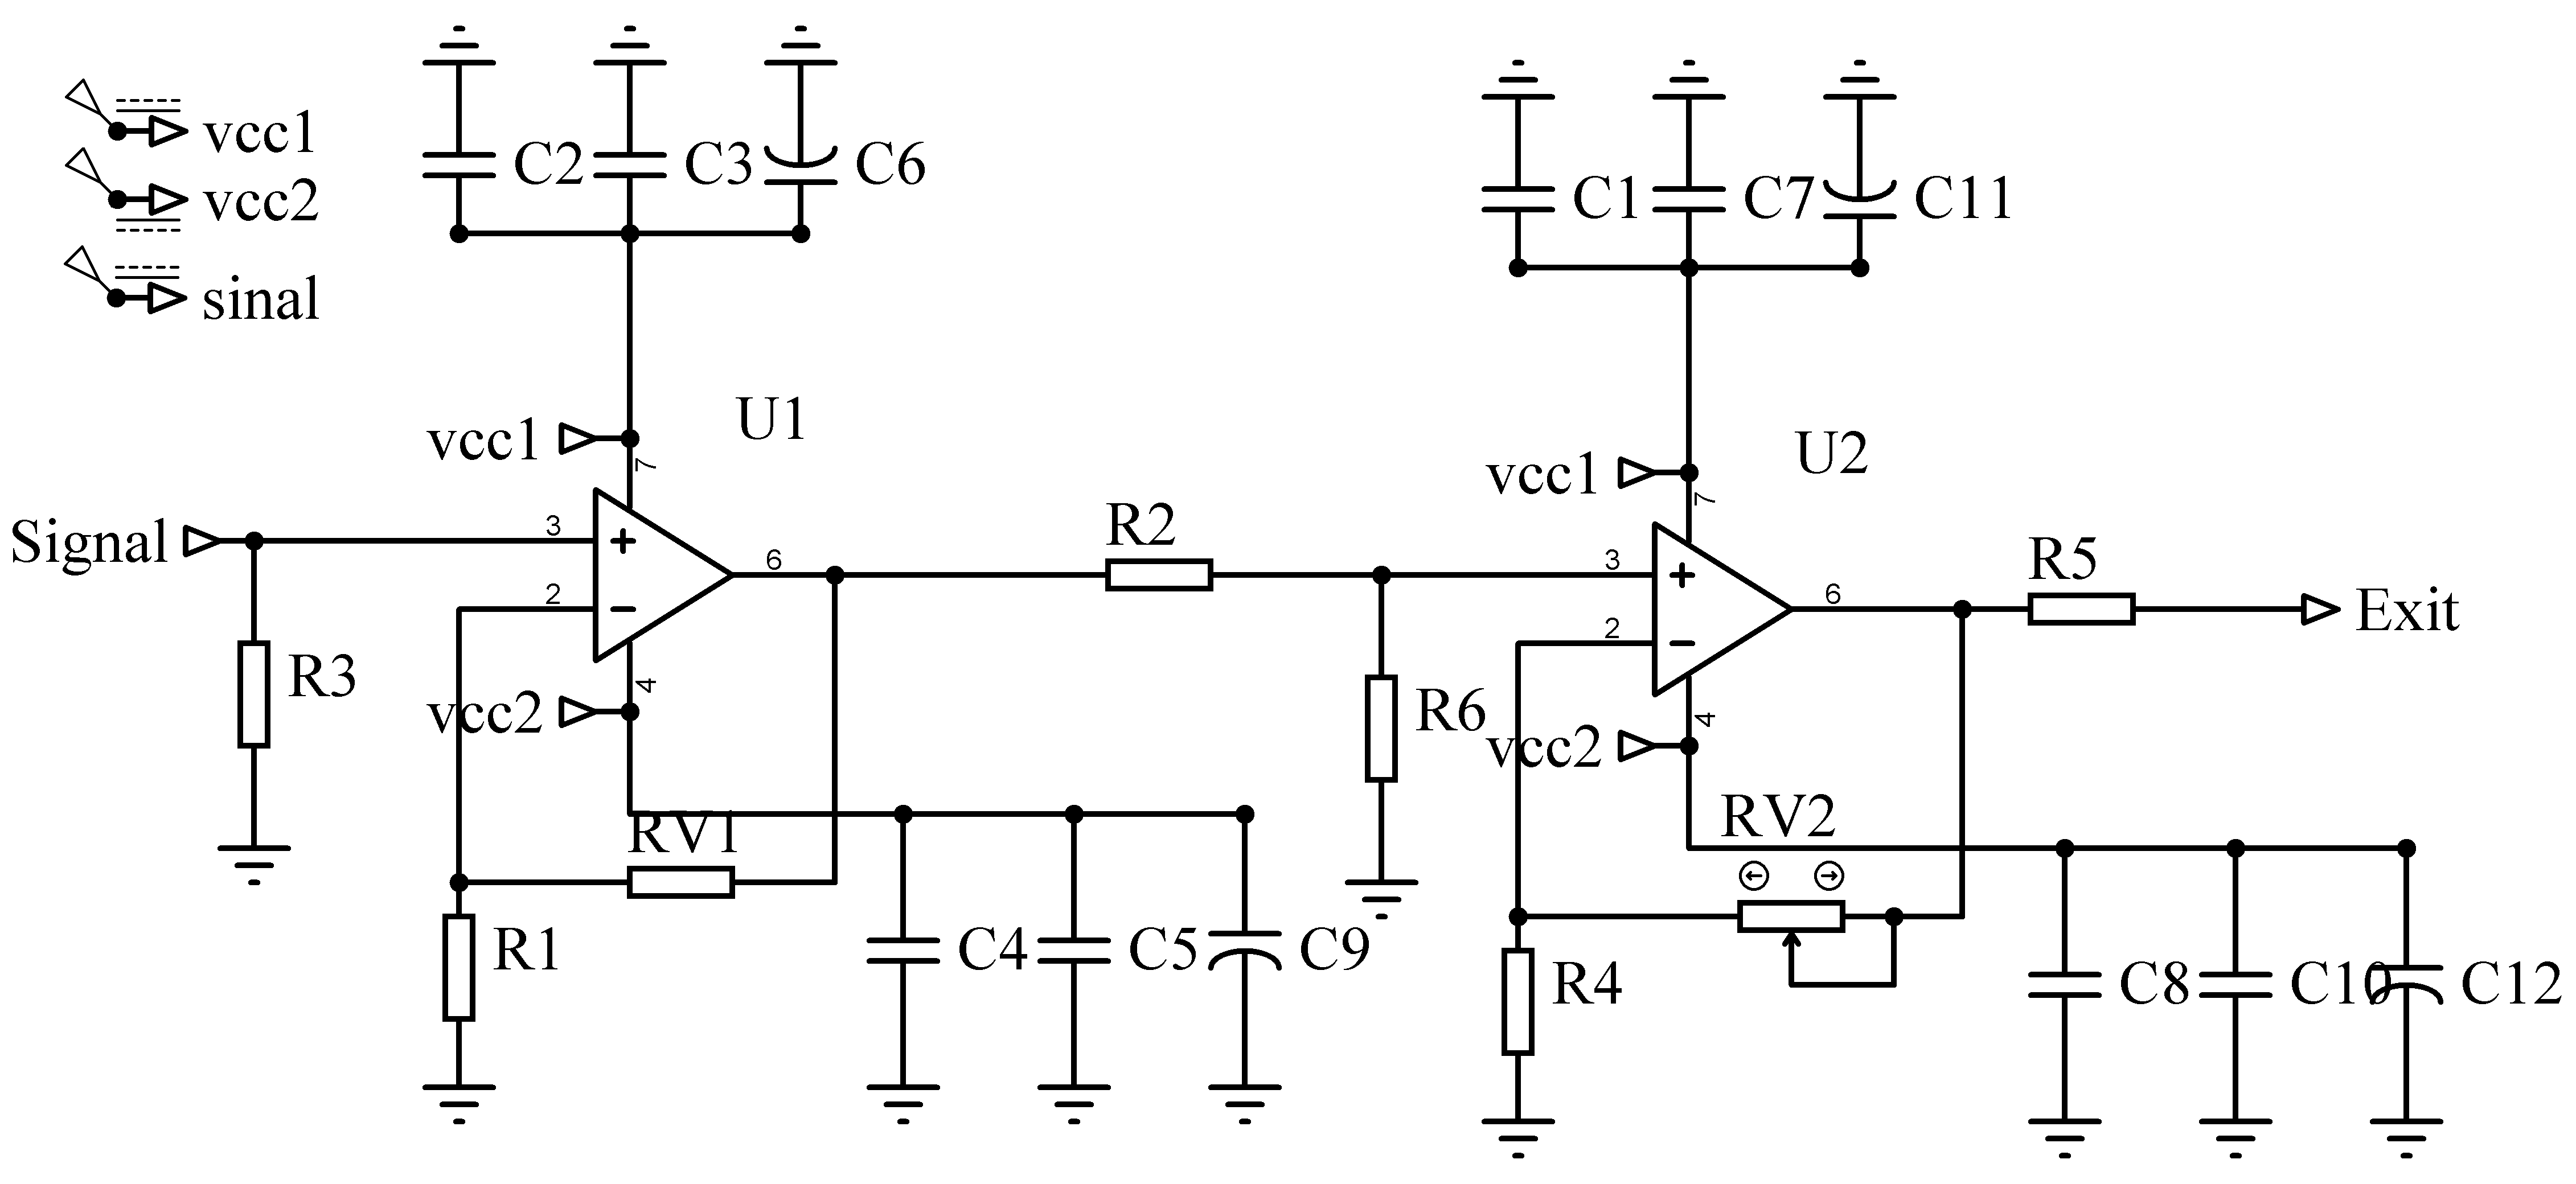
\includegraphics[width=0.9\linewidth]{Figures/SchematicPreamp}
	\caption{Schematic Diagram Pre-Amplification Module}
	\label{fig:7}
\end{figure}

The second module (Fig.\ref{fig:8}) of the circuit refers to the final amplification phase, responsible for generating a signal with known and reliable characteristics to the original. This phase should be accountable for delivering a signal with well-defined features concerning its voltage, with low noise and low distortion. This phase aims to raise the voltage level to expected values.

\begin{figure}[H]
	\centering  
	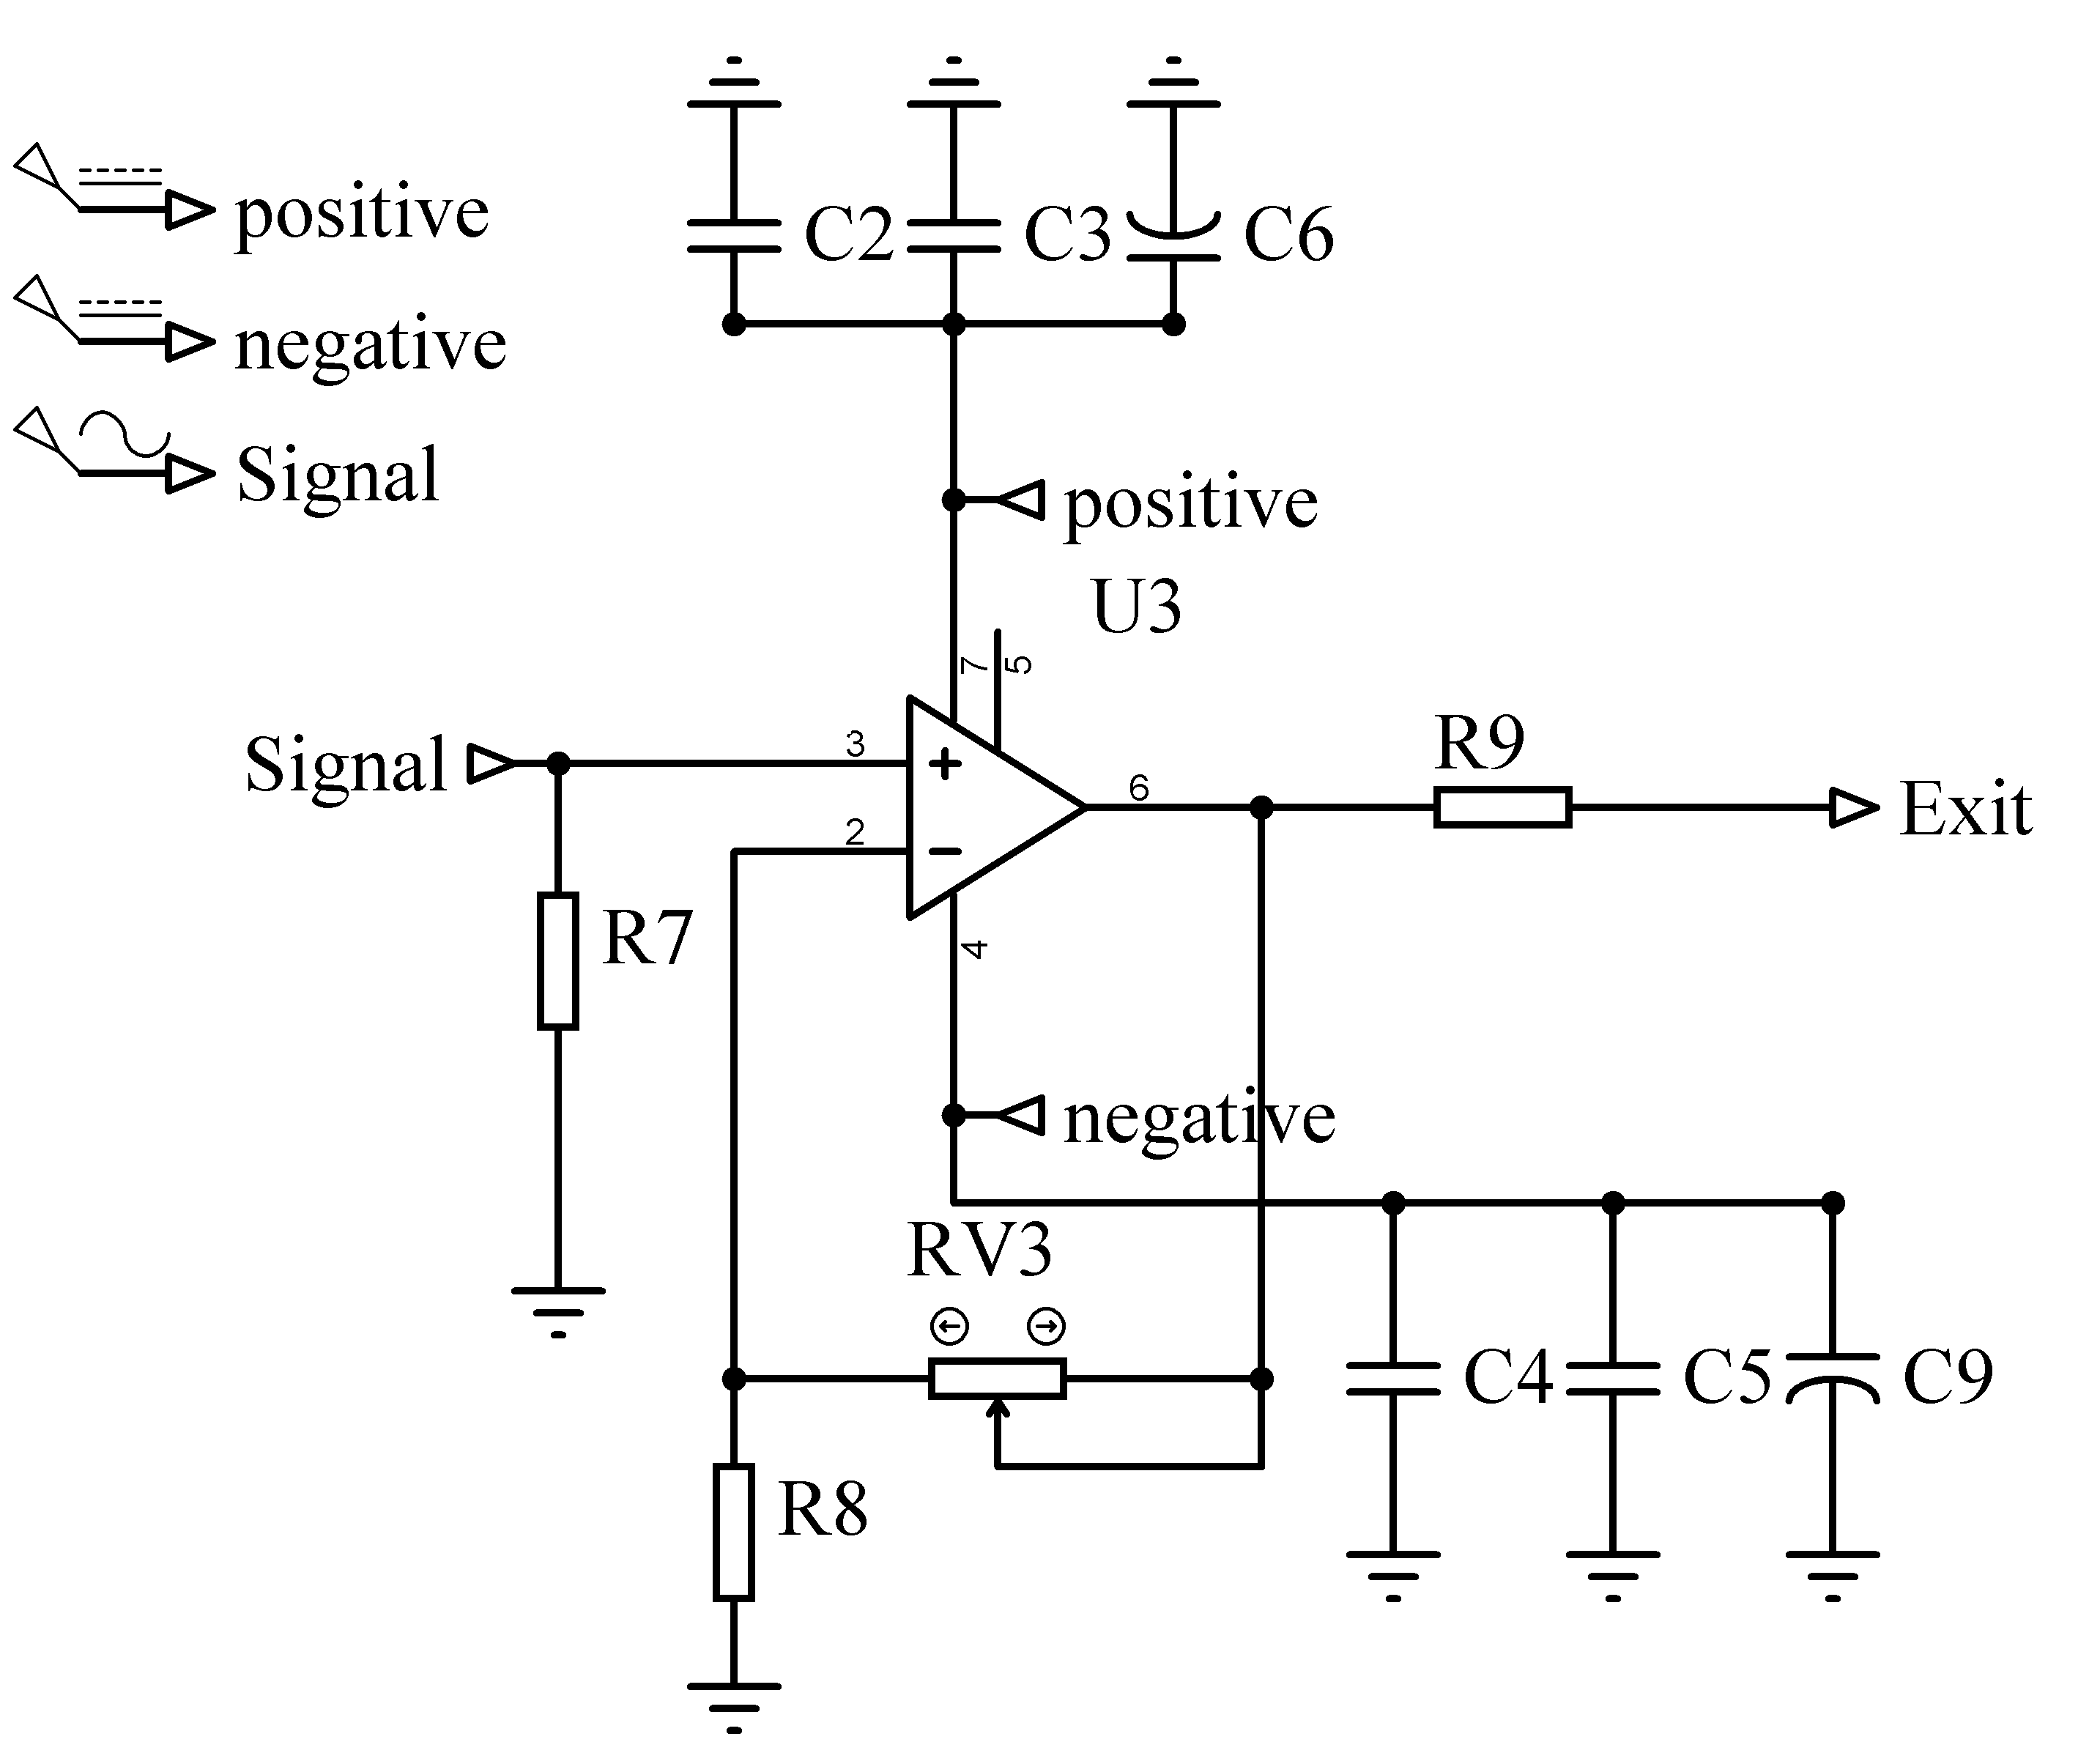
\includegraphics[width=0.6\linewidth]{Figures/SchematicAmp}
	\caption{Schematic Diagram Pre-Amplification Module}
	\label{fig:8}
\end{figure}

The modularized phases of this circuit aim to increase the voltage of a signal. In this way, the initial step is directed towards the minimum increase in voltage necessary for the second amplification phase to detect the signal. In this way, a low-intensity signal can be included in a cascade circuit to acquire characteristics needed for an operation.

Circuits were simulated to visualize their dimensions and constructive characteristics. In this way, the Pre-amplification circuit is presented in Fig.\ref{fig:18}.

\begin{figure}[H]
	\centering  
	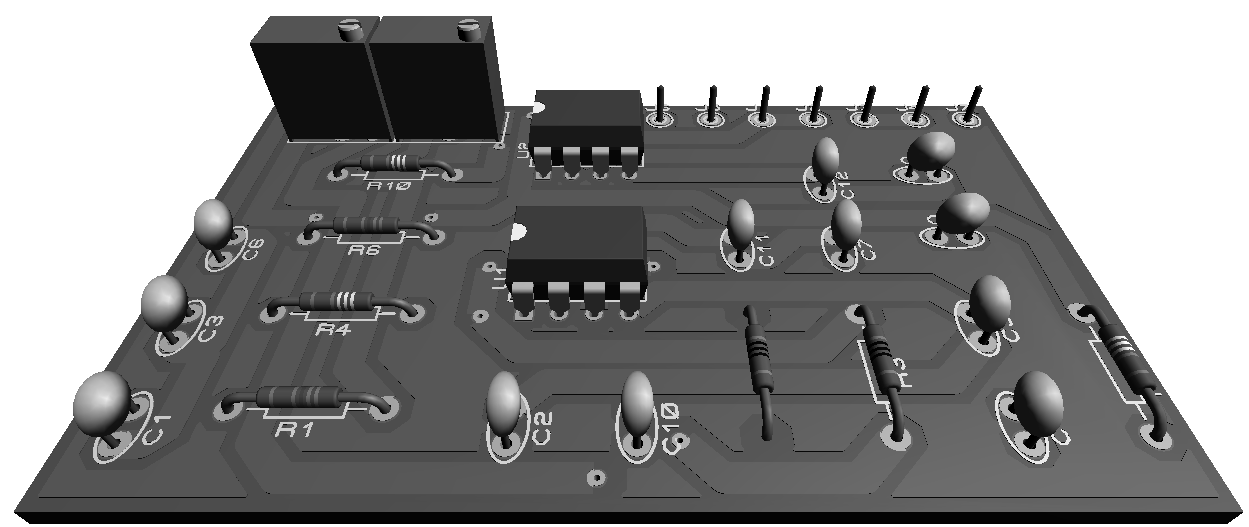
\includegraphics[width=1\linewidth]{Figures/Preamp3D2}
	\caption{Simulated Pre-Amplification Circuit }
	\label{fig:18}
\end{figure}

Like the pre-amplification module, the amplification module was simulated. The structural result of this amplification step is presented in Fig.\ref{fig:19}.

\begin{figure}[H]
	\centering  
	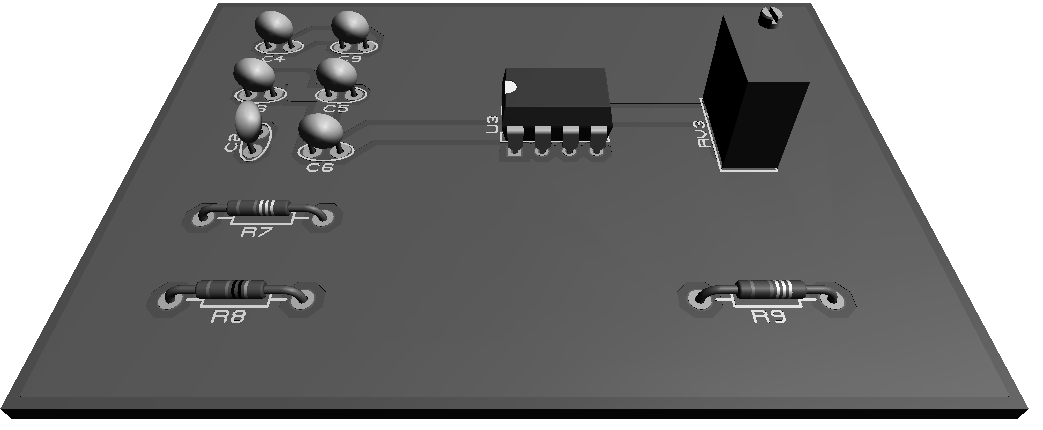
\includegraphics[width=1\linewidth]{Figures/Amp3D2}
	\caption{Simulated Pre-Amplification Circuit}
	\label{fig:19}
\end{figure}

The electronic circuit presented comprises the example case of the application of the methodology. Based on its construction, it is possible to carry out the structure of the FT to model the unavailability of the system based on the failure modes considered. Furthermore, with the quantification of failure rates and the uncertainties involved, it becomes possible to define a model to be considered in the analysis of aging based on the methodological proposal. The quantification of these values must be presented in the following subsection.

\subsection{Failure Data and PCA Criteria}

To exemplify the application of the methodology, the Tab.\ref{table:2} concentrates the values considered, as well as the associated failure modes, as a basis for the choice of system components. Consideration of the failure modes was performed to assess the loss of output signal parameters based on the electronic circuit components' failure.

\begin{table}[H] 
	\caption{Circuit Components Data}
	\label{table:2}
	\begin{center}
		\resizebox{125mm}{!}{
			{\begin{tabular}{@{}ccccccccc@{}}\toprule
					\\
					Component & Failure Mode& $\eta \hspace{2pt}(H)$&$\beta<1^{c}$& $\beta=1^{c}$&$\beta>1^{c}$&$\gamma$\hspace{2pt}$(H)^{e}$\\\\
					\colrule\\
					\multicolumn {1}{l}{Resistor}& \multicolumn {1}{l}{Accuracy Loss}&$M=1540^{a}$&$M=0.3;U_{std}=0.05$&$M=1; U_{std}=0.02$&$M=170; U_{std}=0.05$&0.1\\\\
					\multicolumn {1}{l}{Variable Resistor}&\multicolumn {1}{l}{Position Failure}&$M=1535; U_{std}=25^{b}$&$M=0.3;U_{std}=0.05$&$M=1;U_{std}=0.02$&$M=150; U_{std}=0.02$&0.1\\\\
					\multicolumn {1}{l}{Integrated Circuit}&\multicolumn {1}{l}{Operation Failure}&$^{d}$&$M=0.3;U_{std}=0.05$&$M=1;U_{std}=0.02$&$M=175;U_{std}=0.04$&0.1\\\\
					\botrule
		\end{tabular}}}
	\end{center}
	\footnotesize{$^{a}$ t-student distribution with $scale=20$, Number of Freedom $(NOF)=40$ and confidence interval of 95\%.}\\	
	\footnotesize{$^{b}$ Rectangular distribution.}\\
	\footnotesize{$^{c}$ Gaussian distribution.}\\	
	\footnotesize{$^{d}$ Type A: t-student distribution with $Mean (M) = 852$, $scale= 15.8$ and $NOF= 100$.}\\
	\footnotesize{$^{d}$ Type B: Rectangular distribution with $Mean=695$ and $Standard \hspace{2pt} Uncertainty (U_{std}) =35$.}\\
	\footnotesize{$^{e}$ Location Parameter adopted as constant during the analysis.}
\end{table}

Regarding the application of the PCA, the results obtained with FV should be considered a basis for constructing the model. For this, they must be pre-processed. Among the pre-processing techniques, the scaling method can generate more compatible results with failure analysis para a proposed approach, given its ability to handle data with large dispersions, usually one order of magnitude higher. This pre-processing technique involves applying the centering process in the mean and subsequent processing with the scale technique.

\section{Results and Discussions}

All the results to be presented in that respective section refer to the coverage interval of ninety-five percent.

The first result to be considered is the definition of the FT, which results from the knowledge regarding the functioning of the circuits presented in Fig.\ref{fig:7} and Fig.\ref{fig:8}. Besides, the failure scenario is modeled on the loss of control over a maximum amplified signal configuration of the circuit due to component failures. Based on this, the obtained FT is presented in the Fig.\ref{fig:9}.

\begin{figure}[H]
	\centering  
	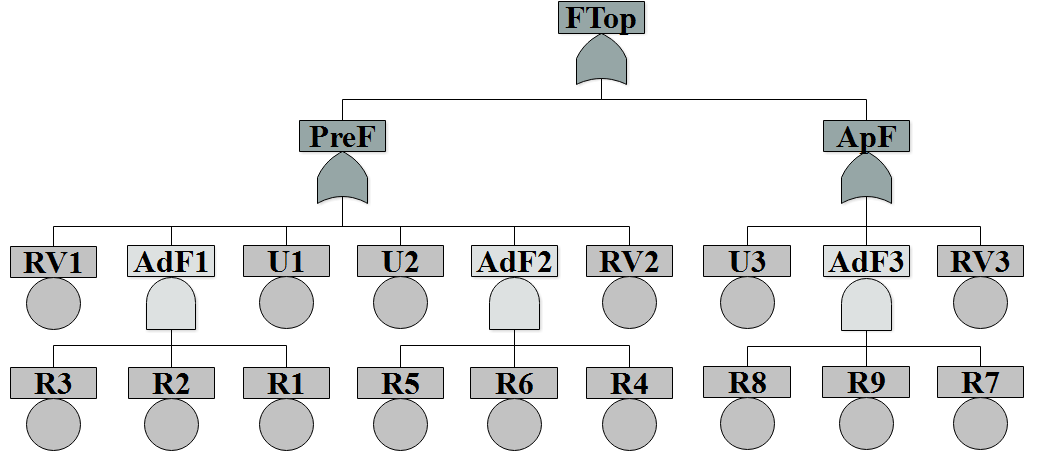
\includegraphics[width=0.95\linewidth]{Figures/FaultTree}
	\caption{Amplification Circuit Failure Tree}
	\label{fig:9}
\end{figure}

The FT presented in Fig.8 has events related to the circuit resistors (R tag), variable resistors (RV tag) and integrated circuits (U tag). Also, it has gates for adjustment failure (AdjF tag), pre-amplification circuit general failure of (PreF tag) and amplification circuit general failure (ApF tag)). Also, it has gates for adjustment failure (AdjF tag), the general flaw of the pre-amplification circuit (PreF tag) and a gate amplification circuit (ApF tag).the FT result is presented by top event gate (FTop tag), that symbolizes the failure of the circuit. It is considered as the inability to maintain the fidelity of an amplified signal with pre-established characteristics. Still in relation to the FT presented, its literal form is obtained through Eq.\ref{eq:8.1}, which indicates the failure probability by considering the failure probability of each component. 

\begin{equation} \label{eq:8.1}
\begin{split}
P(FTop) & =[P(R_{1})P(R_{2})P(R_{3})]+P(RV_{1})+P(U_{1})+P(U_{2})+P(RV_{2})\\
&+[(P(R_{4})P(R_{5})P(R_{6})]+P(U_{3})+P(RV_{3})+[P(R_{7})P(R_{8})P(R_{9})]
\end{split}
\end{equation}
\hspace{2pt}

It is essential to mention that the equation presented does not consider the failures of the capacitors that make up the analysis system. The exclusion of these components is since they are filters for the power supply system, having no impact on the failure analysis model. In this sense, the analysis of these components is more pertinent in analyzing the aging of sources used in the supply of the presented circuit. 

Through the application of the Mc method in Eq.\ref{eq:8.1} and considering the data from Tab.\ref{table:2}, it is possible to perform the aging analysis of the circuit described in the fault tree shown in Fig.\ref{fig:9}, which refers to the system composed of the circuits shown in Fig.\ref{fig:6} and Fig.\ref{fig:7} . 

Eq.\ref{eq:8.1} was processed using the MC method for an analysis time interval of one thousand five hundred and fifty days with a time step of ten days. Each time step was processed by generating five million random numbers. With this processing, the behavior of the probability of failure of the system susceptible to aging is shown in Fig.\ref{fig:10}.

\begin{figure} [H]
	\centering
	\includegraphics[width=0.75\linewidth]{"Figures/Circuit Failure Probability"}
	\caption{System Failure Analysis Results}
	\label{fig:circuit-failure-probability}
	\label{fig:10}	
\end{figure}

Fig.\ref{fig:10} comprises a perfect bathtub curve model. Particular attention should be directed to region three. The uncertainty in this region increases exponentially and can generate failure probability values compatible with part two, which presents the probability of failures with little variation. Another interesting consideration is the behavior of the likelihood of failure in region two of Fig.\ref{fig:10}. The associated uncertainty doesn't have constant behavior, different from what is pointed out in the literature. The fact is presented in \ref{fig:11}.
  
\begin{figure} [H]
	\centering
	\includegraphics[width=0.75\linewidth]{"Figures/Circuit Failure Probability Regiao 2"}
	\caption{Variation in the Constant Fault Region of the Bath Curve}
	\label{fig:circuit-failure-probability-regiao-2}
	\label{fig:11}	
\end{figure}

Although region two is considered an area of constant failures, it has a variation in the probability of failure of a system or component. Even though this variation is present during the analysis, it is small compared to the other analysis regions, making it possible to consider it frequently. This approach also allows this region to be described using the PDF of the exponential distribution.

In addition to the failure study, an in-depth analysis was carried out around the system failure components' percentage participation. This analysis was done using the FV Technique. The technique's processing was carried with MC method considering the same premises involved in studying the system failure. Based on this, three different graphs were obtained concerning the percentage participation for the loss, where each one points to one of the components presented in Fig.\ref{fig:9}. 

The first analysis graph for the contribution to the failure unavailability, taking into account the aging of the system and the associated uncertainties, is directed to the resistor's analysis. The graphic mentioned is shown in Fig.\ref{fig:12}. 

\begin{figure} [H]
	\centering
	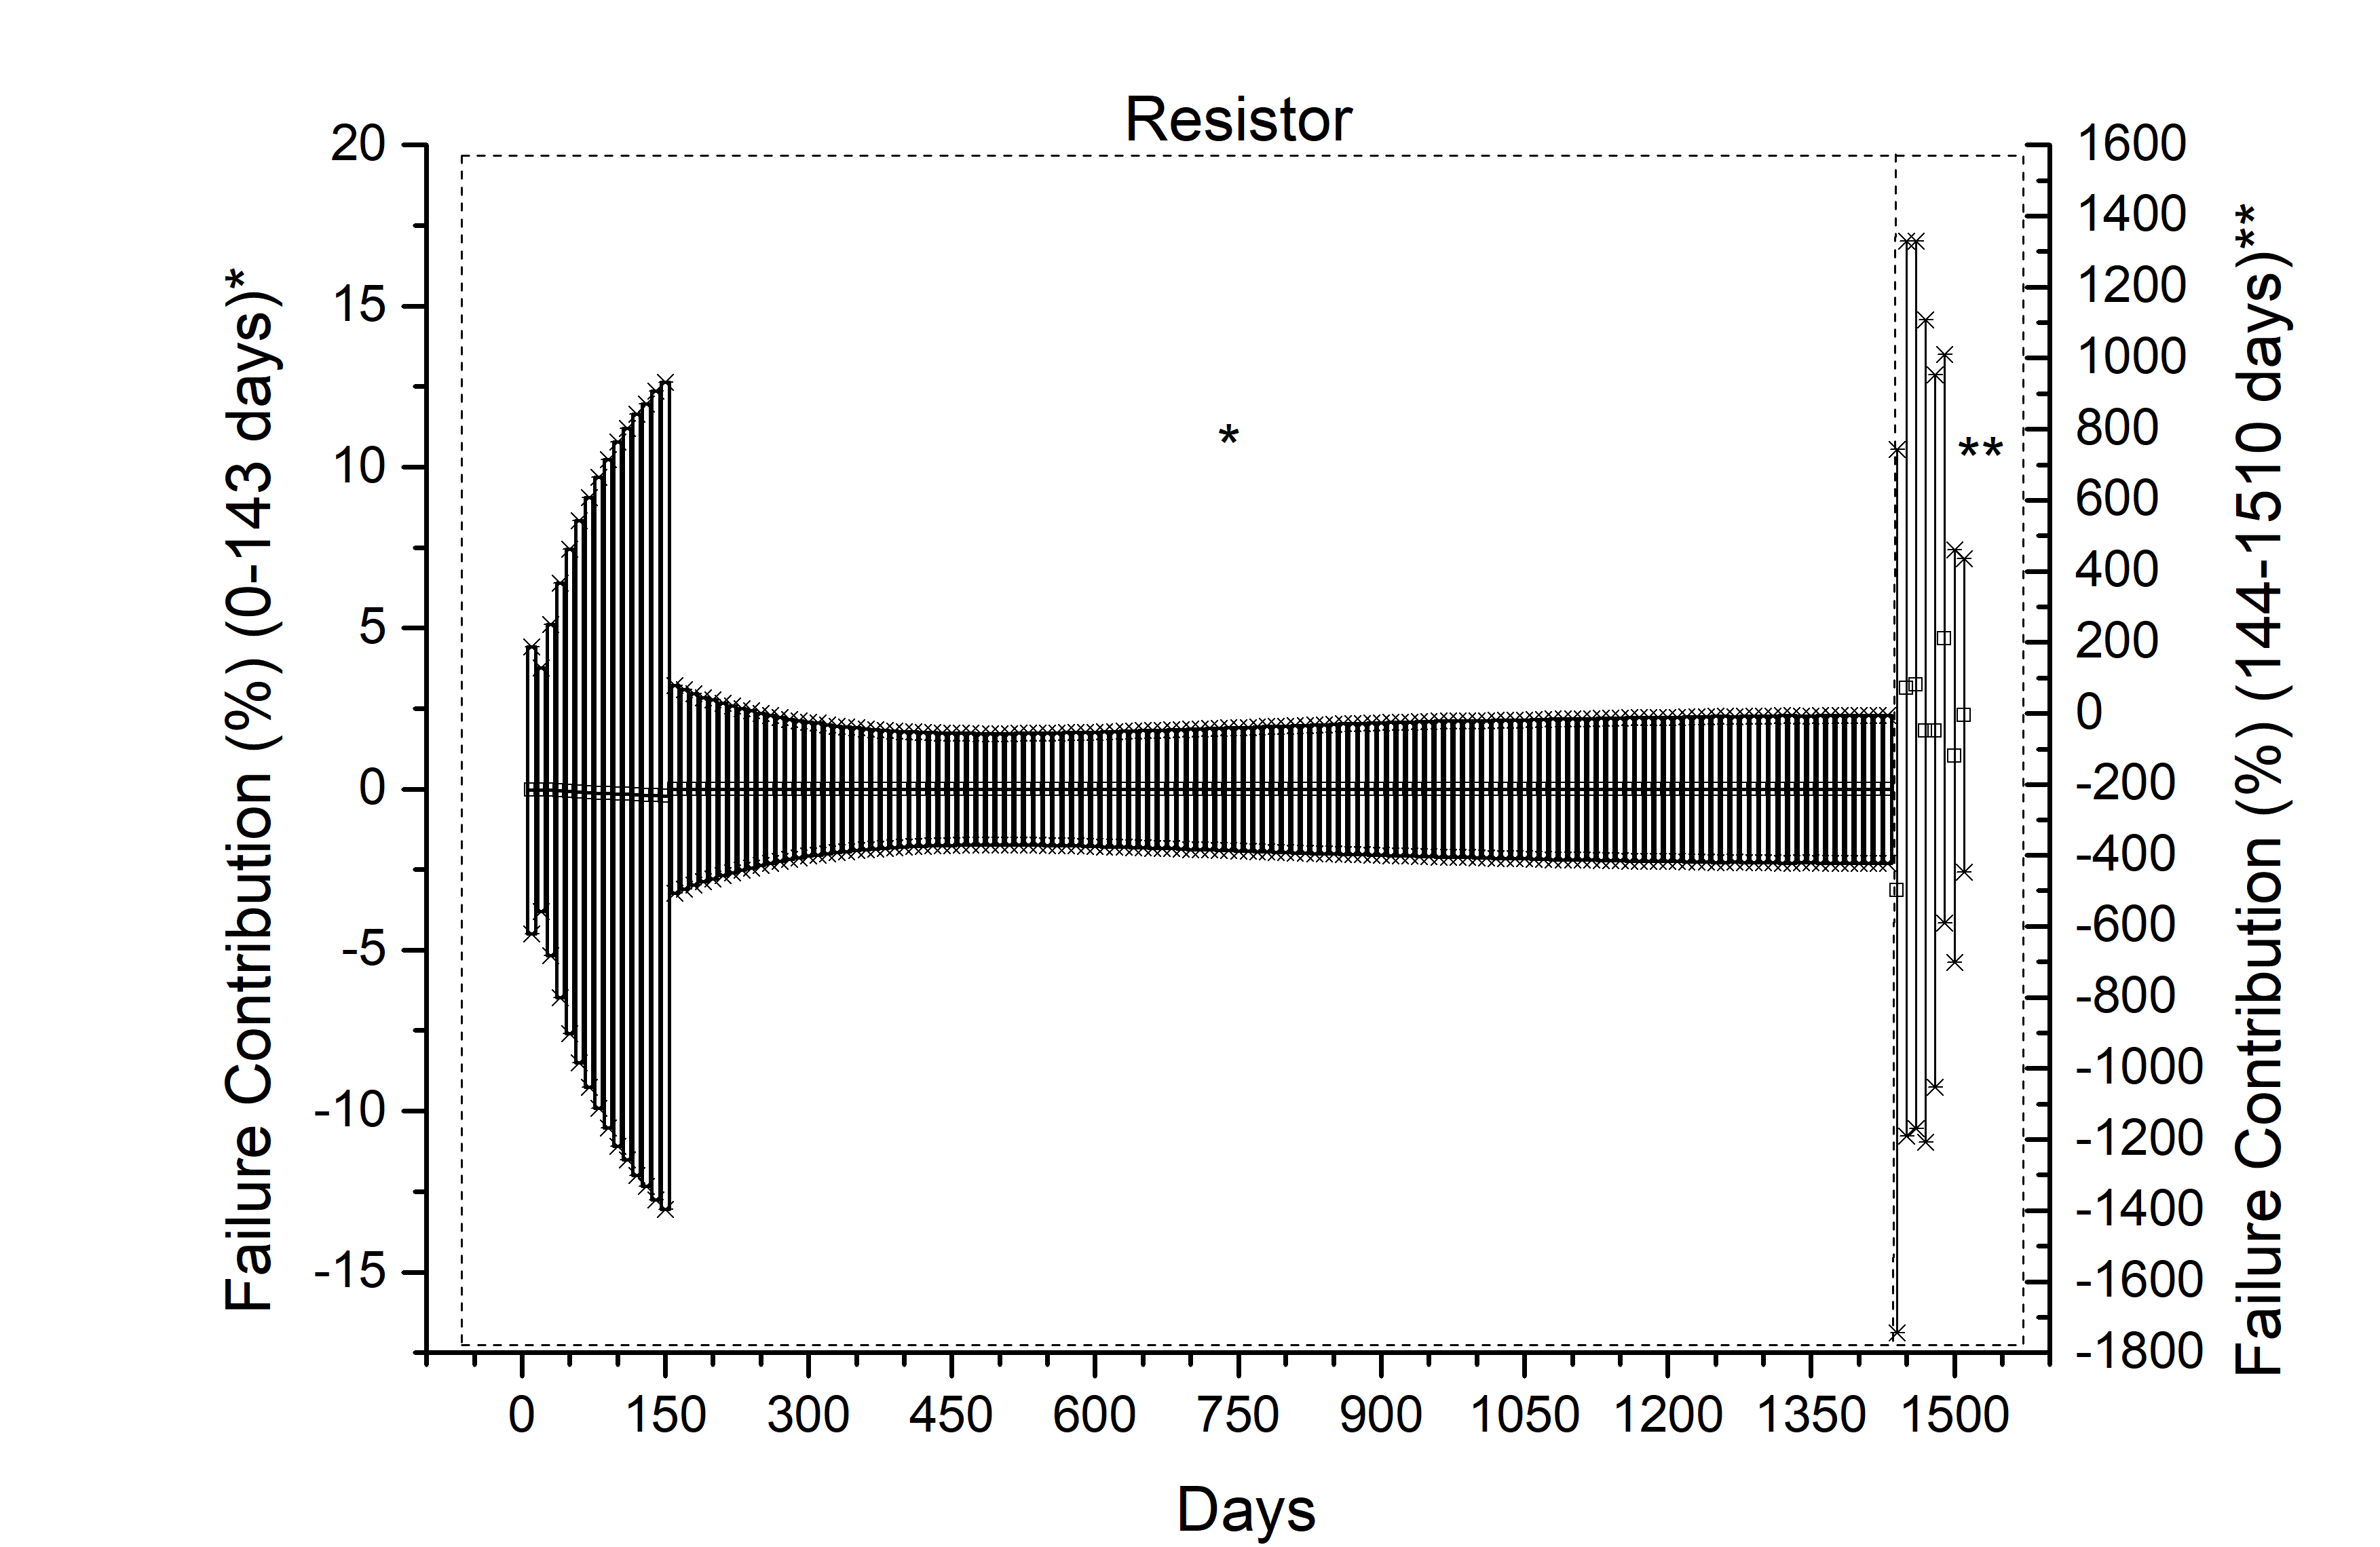
\includegraphics[width=0.8\linewidth]{Figures/RFFull}
	\caption{Failure Contribution (Resistor)}
	\label{fig:rffull}
	\label{fig:12}	
\end{figure}
 
Through the results obtained, the resistor is the component that least contributes to the failure of the amplification circuit. Besides, the average value of the probability of failure is not constant and has a wide variation in the region of exponential increase in failures.
 
In comparison with the previous graph (Fig.\ref{fig:12}), the contribution to the failure by the variable resistor does not remain constant over the analysis time. Therefore, there is a variation in the average value of contributions.

The variable resistor presents itself as one of the most significant components for the system's unavailability, showing greater relevance for the unavailability of the system over the analysis time, whose contribution to the system failure is shown in Fig.\ref{fig:13}.

\begin{figure} [H]
	\centering
	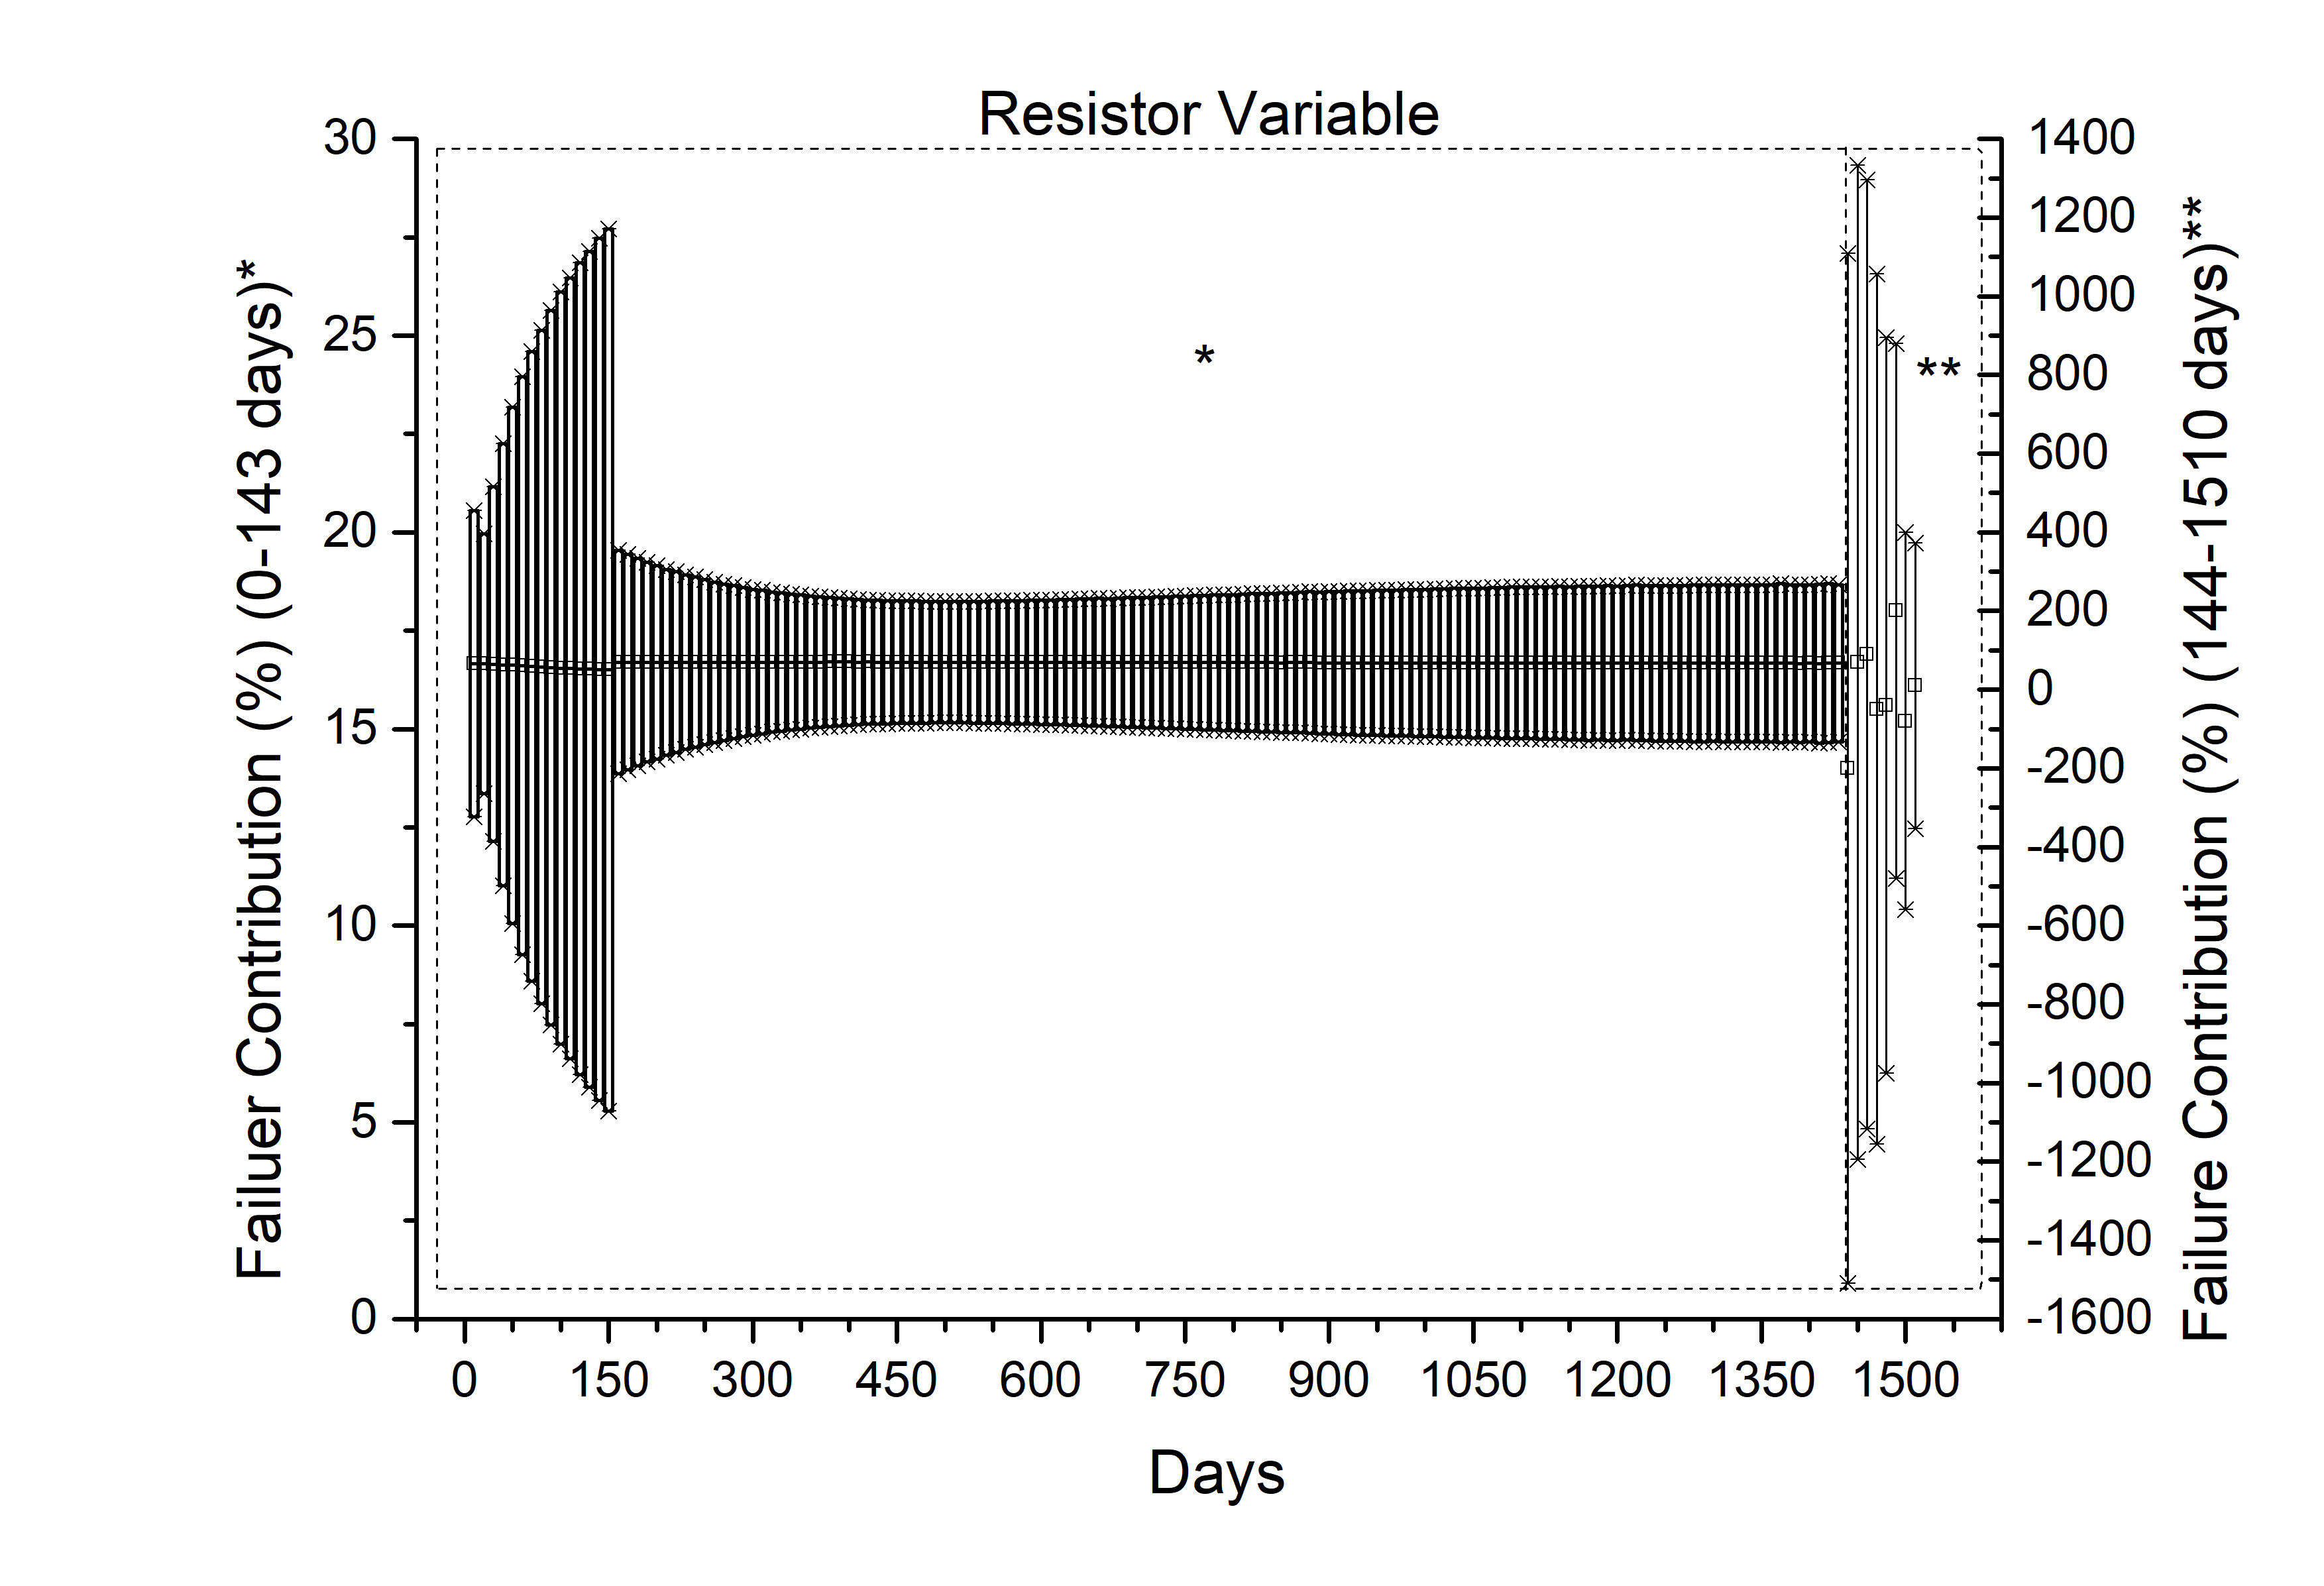
\includegraphics[width=0.8\linewidth]{Figures/RVFull}
	\caption{Failure Contribution (Variable Resistor)}
	\label{fig:rvfull}
	\label{fig:13}
\end{figure}

The last component to be analyzed is the Integrated Circuit, which contributes to the unavailability of the equivalent resistor system. The analysis for the percentage contribution of the component is presented in Fig.\ref{fig:14}.

\begin{figure} [H]
	\centering
	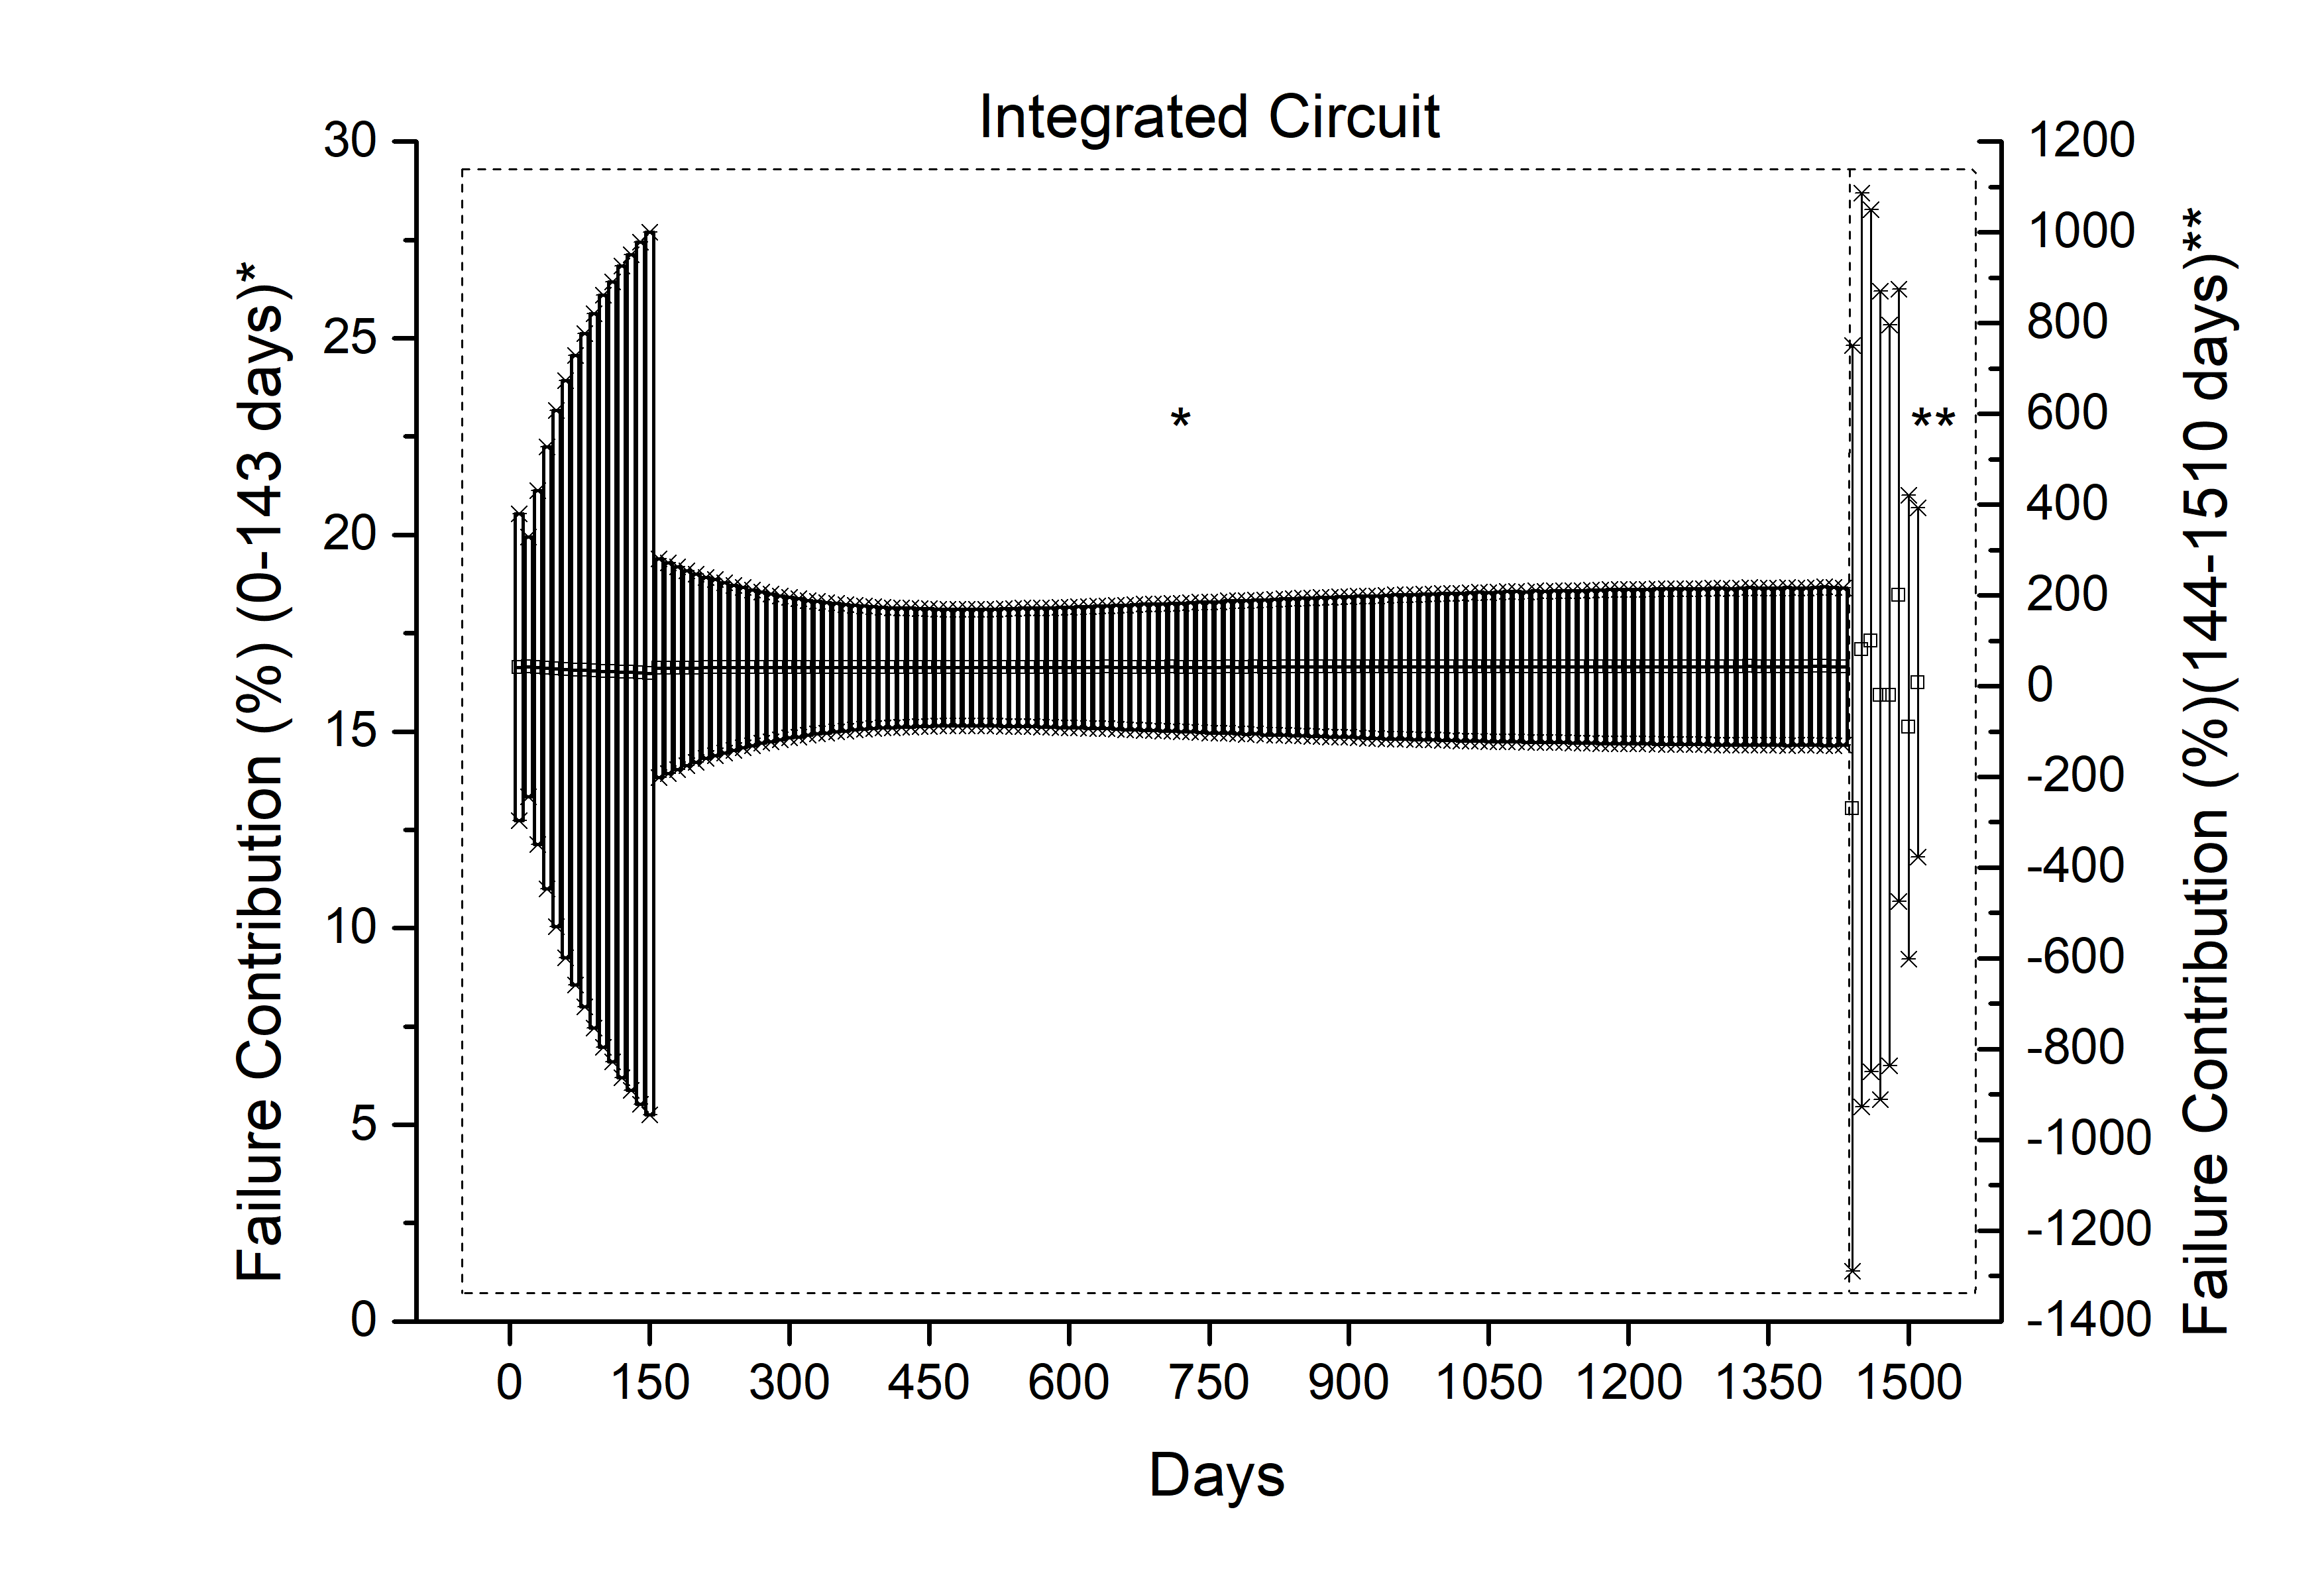
\includegraphics[width=0.8\linewidth]{Figures/ICFull}
	\caption{Failure Contribution (Integrated Circuit)}
	\label{fig:icfull}
	\label{fig:14}
\end{figure}

The similarity with the participation in the system failure through the Integrated Circuit and the Resistor Variable can be explained by the mathematical operators associated with these components and their position in the fault tree. These components are the most participatory for the system's unavailability, unlike the resistor, which has low participation. 

Regarding the exponential increase in failures, it is essential to highlight the fact that anomalies appear at the beginning of this region, indicating that the participation of the components has extreme values in this region.

Analysis using the FV technique can generate countless results that can be difficult to visualize graphically. Thus, PCA can present itself as an essential tool for the composition of a model that can be visualized as the information can be inserted and analyzed with the contribution of components to the system's failure.

By using the values obtained with FV, with the scaling processing technique, and the application of the PCA, the contribution to the components' failure can be seen more simply. Thus, it is necessary to compose graphs pertinent to the technique, e.g., score graphs and loadings (Fig.\ref{fig:16}).The comparison between these graphs makes it possible to determine the most remarkable correlation between components and time passages. This analysis generates results similar to those presented in the previous graphs on the contribution of components to the electronic circuit's unavailability.

Based on the analysis of the contribution to the system's unavailability concerning its components, components that have a more significant contribution to the system's failure generate greater uncertainties, as well as the anomaly perceived at the beginning of the exponential increase in system failure.

\begin{figure}[H]
	\centering
	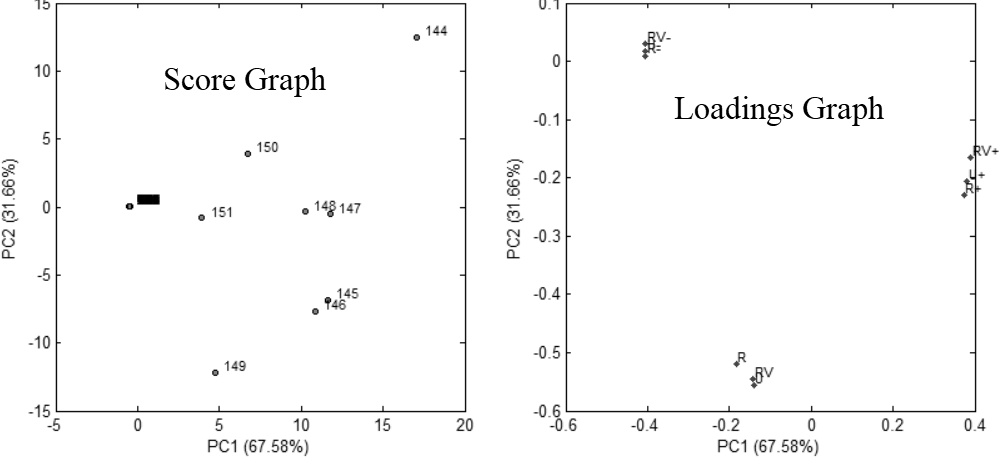
\includegraphics[width=1\linewidth]{Figures/ScorexLoadings.png}
	\caption{Score and Loadings Graphics}
	\label{fig:fvloadings}
	\label{fig:16}
\end{figure}

Still using the PCA, a dendrogram can be created to verify the compatibility between the components, e.g., which can be grouped according to the participation for the system's unavailability. In this way, Fig.15 presents the dendrogram referring to the aging analysis of the system.

\begin{figure} [H]
	\centering
	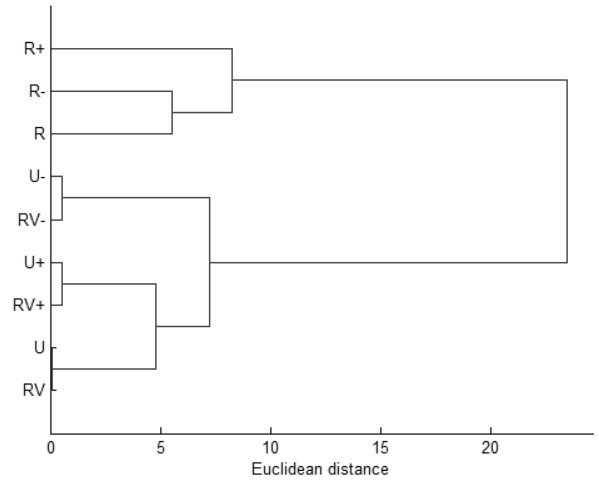
\includegraphics[width=1\linewidth]{Figures/FVDendogram}
	\caption{System Dendogram}
	\label{fig:fvdendogram}
	\label{fig:17}
\end{figure}

The graphs presented in Fig.\ref{fig:16} present components considered in the FT of the analysis case and are pointed out through combinations of their first letters. Furthermore, uncertainties are considered, being presented using their upper limit, indicated by the symbol $(+)$, and the lower limit, indicated by the symbol $(-)$.
	
\section{Acknowledgment}

I am grateful for the help and cooperation of the Instituto Nacional de Metrologia, Qualidade e Tecnologia (INMETRO), the Instituto de Engenharia Nuclear (IEN) and the Fundação de Amparo à Pesquisa do Estado do Rio de Janeiro (FAPERJ), which contributed to the work presented in this paper has been carried out.

\section{Conclusions}

The concepts and techniques used in the development of the proposed aging analysis methodology are known in the literature, mainly in failure analysis applications, except for PCA, whose application is a pioneer in failure analysis. The everyday use of these tools makes it possible to obtain relevant results in an aging study. Additionally, the consideration of the associated uncertainties pointed out that it is capable of generating results that make it impossible to compose a predictive model that describes the reality of the system concerning aging.

The methodology proposed in this work, refers to using high production analysis tools, thus generating the expectation of developing predictive models, which can be formed in real-time with any given system. In this perspective, it is essential to mention that a proposal presented throughout this role can be applied in several types of systems, its application being critical in installations that require high reliability, such as a nuclear, aerospace industry, for example.

Regarding the analyzed circuit, it was found that the variable resistor and the integrated circuit are the most sensitive components of the system, being responsible for the most outstanding contribution to the unavailability of the system. This determination points to decision-making measures that can impact the increase in the system's reliability, such as replacing them based on the circuit design or over the time of operation.

The methodology for the analysis of aging throughout this paper enables the modeling, analysis of aging and a clear presentation of a system's analysis data throughout its operation. In this way, the methodology is relevant for failure studies and presents itself as contributing to the increase in reliability and system availability guarantees.


\begin{thebibliography}{0}
	
%1
\bibitem{WenyuanLi2006}Wenyuan Li and E. Vaahedi and P. Choudhury, Power system equipment aging, {\it IEEE Power and Energy Magazine} {\bf 3} (2006) 52--58.

%2
\bibitem{Klutke2003}G. Klutke and P.C. Kiessler and M.A. Wortman, A critical look at the bathtub curve, {\it IEEE Transactions on Reliability} {\bf 1} (2003) 125--129.

%3
\bibitem{Matsuoka2012}Matsuoka Takeshi, Failure data and system reliability analysis, {\it Nuclear Safety and Simulation} {\bf 2} (2012) 104--118.

%4
\bibitem{VIM2012}Bureau International des Poids et Mesures (BIPM), International Vocabulary of Metrology -  Basic and General Concepts and Associated Terms (JCGM 200:2012) {\it BIPM} {\bf 1} (2012) 1--95.

%5
\bibitem{Borges2015}Borges, Diogo S. {\it et all}, Nondeterministic method to analysis of the aging effects in PWR power plants components {\it Annals of Nuclear Energy} {\bf 81} (2015) 249--256.

%6
\bibitem{Epin2002}Marko {\v{C}}epin and Borut Mavko, A dynamic fault tree {\it Reliability Engineering {\&} System Safety} {\bf 1} (2002) 83--91.

%7
\bibitem{Lai2006}Chin-Diew Lai and D.N. Murthy and Min Xie, Weibull Distributions and Their Applications {\it Springer Handbook of Engineering Statistics} {\bf 1} (2006) 63--78.

%8
\bibitem{Gupta2010}Arjun K. Gupta and Wei-Bin Zeng and Yanhong Wu, Exponential Distribution {\it Probability and Statistical Models} {\bf 1} (2010) 23--43.

%9
\bibitem{Rinne2008}Horst Rinne, The Weibull Distribution {\it Chapman and Hall/{CRC}} {\bf 1} (2008) 01--92.

%10
\bibitem{Yoriyaz2009}Hélio Yoriyaz, Monte Carlo Method: principles and applications in Medical Physics {\it Revista Brasileira de Física Médica} {\bf 1} (2014) 141--149.

%11
\bibitem{GUN2008}Antonio Carlos Baratto, Jailton Carreteiro Damasceno, João Antonio Pires Alves, Jorge Trota Filho, Paulo Roberto Guimarães Couto and Sérgio Pinheiro de Oliveira, Avaliação de dados de medição — Guia para a expressão de incerteza de medição {\it JCGM 100:2008} {\bf 1} (2008) 01--138.

%12
\bibitem{Shadiah2019}H. M. Nor Shadiah and Ahmad Arshad and A. R. Khalil Mohamed and Oladokun Olagoke, Integration of fault tree and importance measure for toxic prevention barrier {\it E3S Web of Conferences} {\bf 90} (2008) 02007.

%13
\bibitem{vanderBorst2001}M van der Borst and H Schoonakker, An overview of {PSA} importance measures {\it Reliability Engineering {\&} System Safety} {\bf 3} (2001) 241--245.

%14
\bibitem{Mishra2017}Sidharth Mishra and Uttam Sarkar and Subhash Taraphder and Sanjoy Datta and Devi Swain and Reshma Saikhom and Sasmita Panda and Menalsh Laishram, Principal Component Analysis {\it International Journal of Livestock Research} {\bf 3} (2017) 01--20.

%15
\bibitem{Tharwat2016}Alaa Tharwat, Principal component analysis - a tutorial {\it International Journal of Applied Pattern Recognition} {\bf 3} (2017) 01--142.

%16
\bibitem{Adcock2015}Adcock, Jeremy and Allen, Euan and Day, Matthew and Frick, Stefan and Hinchliff, Janna and Johnson, Mack and Morley-Short, Sam and Pallister, Sam and Price, Alasdair and Stanisic, Stasja, Advances in quantum machine learning {\it Advances in quantum machine learning} {\bf 1} (2015) 01--37.

%17
\bibitem{vandenBerg2006}Robert A van den Berg and Huub CJ Hoefsloot and Johan A Westerhuis and Age K Smilde and Mariët J van der Werf, Centering,  scaling,  and transformations: improving the biological information content of metabolomics data, {\it {BMC} Genomics} {\bf 1} (2006).

%18
\bibitem{Parente2013}Alessandro Parente and James C. Sutherland, Principal component analysis of turbulent combustion data: Data pre-processing and manifold sensitivity {\it Combustion and Flame} {\bf 2} (2013) 340--350.

%18
\bibitem{Han2012}Han, Jiawei, Data mining : concepts and techniques {\it Elsevier/Morgan Kaufmann} {\bf 1} (2012) 01--740.

\end{thebibliography}

\end{document}

%%Typeout the superscript citation as:-
%%(1) word,\cite{aiz,am,lar} and word.\cite{aiz,am,lar}
%%(2) word\cite{ba}: word\cite{ba}; word\cite{ba}?
%%(3) See Ref.~\refcite{lar} --- to be cited at the text.
